\chapter{Optics I: Reflection, Refraction, and Lens Equation}

\section{Introduction}

This experiment is the first of two experiments introducing the basic ideas of geometrical optics. These experiments will introduce you many new physics concepts so it is important to read the theory section before your lab section. \footnote{The material in these labs is discussed in the assigned lecture course textbook (Fundamentals of Physics, 10th Ed., Halliday, Resnick \& Walker, Chapters 34-38) In particular, we adopt the sign conventions used in the course textbook.}  They are designed to present the ideas of geometrical optics from an empirical point of view.\myskip

In this first experiment, we utilize a simple model describing light as a bundle of rays.  We then explore the behavior of these rays as they reflect from smooth surfaces and as they are transmitted, or refracted, through transparent media.  We will experimentally verify Snell's law of refraction and observe the phenomenon of total internal reflection as a consequence of Snell's law.\myskip

We will subsequently use the concept of light rays to describe ray diagrams and derive the lens equation\footnote{Many approximations are made with ``thin lenses''. However, even the most sophisticated treatments of optics usually begin with these ``thin lens approximations''.}. These are powerful tools to draw conclusions based on geometrical optics. In this experiment, we will verify the lens equation for real and virtual images. In the next experiment, we will use these tools to build a magnifying glass, microscope, and telescope.\myskip

Why is optics important (besides the fact that the human eye works by the rules we describe here)? Optical instruments are used in many real-life situations in which an image of a system is needed.  Such cases apply whether the system is large or small, and whether easily accessible or not.  For example, whenever you want insight into how a biological system works, you will likely need to use imaging methods based on geometrical optics. Even if you are only interested in the final data from some fancy imaging system, it will be essential for the quality of your work that you know how to evaluate what you are seeing and what the limitations of the method are.\myskip

\emph{Remark}: It is strongly recommended that you look over the setup in the Lab Library before coming to the lab. It is difficult to understand optical phenomena in the abstract so simply reading the lab manual might not be enough to fully prepare for this lab.  Be sure to stop by the Lab Library and let the TA show you the apparatus!

\section{Theory}

\subsection{Geometrical Optics}

Geometrical optics is a simplified way of describing light phenomena. It is valid as long as we do not consider cases in which light passes through small pinholes or slits, or examine the edges of shadows. In your lecture and lab this semester, you will encounter effects such as diffraction and interference, which are much more complicated and cannot be accurately explained by the theory of geometrical optics. The assumption for geometrical optics is that rays of light propagate along straight lines until they are reflected, refracted, or absorbed at a surface. \myskip

A very simple, but important, application of geometrical optics is X-rays. (X-rays are a type of `light', with wavelengths that are much shorter than those characteristic of visible light.)  The shadow image of the skeleton made in an X-ray may be understood by simply propagating straight lines from the source to the detector, except for those rays absorbed by some tissue (e.g. bone) in the path.

\subsection{Light as Rays}

The concept of light rays may become more plausible to you if you imagine being in a dark, dusty room with light from the outside entering through a small hole. You can ``see'' a ray of light traveling in a straight line from the hole to wherever it hits the wall.  (Your eye actually sees the light scattered by dust particles along the path of the ray.)\myskip

We describe light using the following simple model. A light source emits rays of light in all possible directions. Each ray propagates along a \emph{straight line} until one of the following happens. It is:
\begin{enumerate}
    \item	reflected if it encounters a reflective material.
    \item	refracted if it encounters a transparent material.
    \item	absorbed if it encounters a non-reflecting, non-transparent material.
\end{enumerate}
For most materials in the real world, combinations of these effects occur.\myskip

\begin{figure}[h]
    \begin{center}
        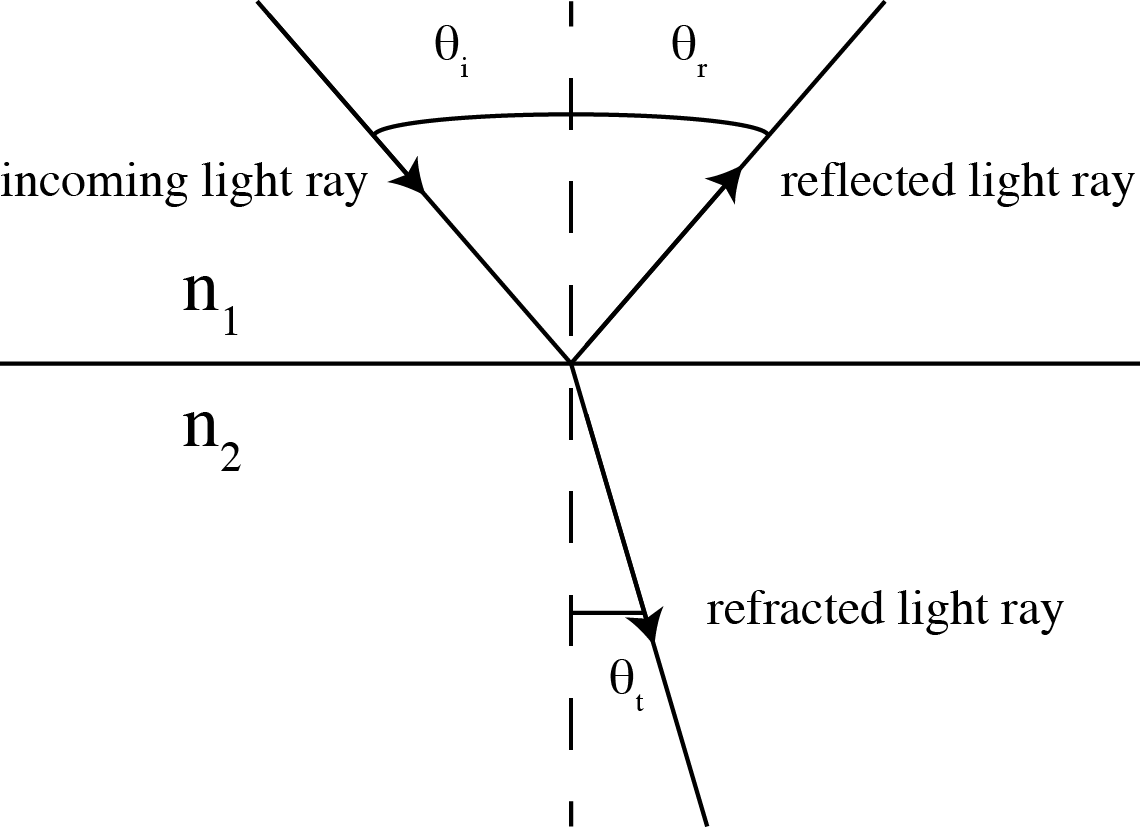
\includegraphics[width=0.5\textwidth]{./Exp6/pic/basicsnelllaw.png}
    \end{center}
    \caption{Reflection and Refraction of Light Ray Across a Surface}
    \label{fig:rayref}
\end{figure}

In geometrical optics, we assume that each ray of light travels along a straight line indefinitely unless it strikes a boundary, like a mirror or an interface between air and another material. A source of light, such as a flashlight, produces many rays that travel nearly parallel to each other on their way to the illuminated spot on the boundary. If a ray is not absorbed when it strikes the boundary, it splits into parts as shown in the figure above. Both the reflected and refracted rays again travel in straight lines until they encounter another boundary. The angles $\theta_{i}$, $\theta_{r}$, and $\theta_{t}$ are measured with respect to the normal (perpendicular) to the boundary surface.\myskip

Although in actuality a light ray that encounters a surface experiences all three of these effects, there is usually one that dominates. If the boundary is a metallic mirror, only the reflected ray is relevant, and if the boundary is a transparent medium such as water, only the refracted ray is relevant. In sections 2.4 and 2.6, we describe the quantitative relationships between the incident ray and the reflected and refracted rays. In particular, we write the relations between the angles $\theta_{i}$ and $\theta_{r}$, and between the angles $\theta_{i}$ and $\theta_{t}$ shown in Figure \ref{fig:rayref}.

\subsection{Absorption/Color (a brief aside)}

The colors we perceive in light are directly correlated with the wavelength of the light ray (for example, blue light has a shorter wavelength than red light). White light is the response your brain perceives if light of all colors strikes your eye's receptors.  \myskip

Materials that absorb light can either decrease the reflected intensity for all colors equally (which means that the light simply appears less bright than before) or they can selectively decrease the intensity of some colors. An example of the second case is white light from the sun falling onto the grass where the grass absorbs all colors except green (which it reflects). This is why grass appears to you as green. If an object absorbs all the light, it appears to be black.\myskip

All materials absorb to some extent, even when the light appears to pass through or reflects. (The best commercial mirrors reflect about 99.99\% of the incoming light.)

\subsection{Reflection}

The ray reflected from a surface emerges at an angle equal to the angle of incidence of the original light ray.  Quantitatively, this law of reflection is expressed in terms of the angles shown in the figure as:
\begin{equation}
    \theta_{r} = \theta_{i}
\end{equation}
There are two general types of reflection -- diffuse and specular. Diffuse reflection is exemplified by the reflection from the surface of this page. On a microscopic scale, the surface of the paper is quite rough; consequently, parallel rays striking even nearby parts of the paper's surface are characterized by different angles of incidence. Each of the initially parallel rays is reflected in a different direction.  Therefore, when we shine a flashlight on a piece of paper, irrespective of our position, we see a bright spot on the paper.\footnote{Only a few of the light rays are reflected into our eyes!}  In this case, it is not feasible to determine the relationship between $\theta_{i}$ and $\theta_{r}$ for any particular ray.\myskip

If parallel rays reflect from a surface which is very flat and smooth (such as that found on a mirror or on window glass), there is a unique angle of incidence and therefore a unique angle of reflection. This type of reflection is referred to as specular or regular. A flashlight beam reflected specularly will only be observed if it is viewed along the direction of reflection. We restrict our attention here to specular reflection, since only in that case the relationship between the incident and reflected rays can be understood well enough to be used in optical instruments.  \myskip

You may have seen fresh snow glitter in the sunlight, and wonder which type of reflection that is. The explanation is that some of the small flat surfaces of the snowflake are smooth and act like mirrors that reflect several rays in the same direction, which just happens to be where your eye is. But the totality of the surface of white snow is irregular and reflection from the snow more often looks much like the diffuse reflection from this page.\myskip

\emph{Remark for Experts}: There is of course no \underline{perfectly} smooth surface in nature. Every surface is rough on the atomic level. To get specular reflection, it is sufficient that surface irregularities are small compared to the wavelength of light. So when you polish anything, from optical instruments to your furniture, the desired successful appearance is accomplished when you have made all surface irregularities small compared to the wavelength of light (which is about $5\times 10^{-5}\,\mathrm{cm}$, or $500\,\mathrm{nm}$). Since atoms are much, much smaller than that, there is no contradiction.

\subsection{Real and Virtual Images}

When you look in a mirror, you see your own image. It looks as if a copy of you is standing behind the mirror. But if you put a screen behind the image at the position where your copy seems to stand, you would obviously not capture the image of yourself on the paper. Your copy in the mirror or any image you cannot capture on a screen at its apparent location is called a virtual image. If you can record the image on a screen at its apparent location, it is called a real image. Real images are caused by the actual convergence of light rays at a given point; virtual images are caused by light rays that diverge in such a way that they seem to, but do not actually, converge at a certain point.\myskip

Mirrors produce virtual images. In the next two labs, we will deal with many different examples of real and virtual images.

\subsection{Refraction and Snell's Law}

Light waves (rays) propagate through vacuum with a fixed velocity $c$ equal to about $300,000\,\mathrm{km/s}$ or $3\times 10^8\,\mathrm{m/s}$. One of the consequences of our understanding of electromagnetism, detailed in Einstein's theory of special relativity, is that nothing can travel faster than this speed.  \myskip

As the waves travel through any material, interactions of the light with the atoms result in a velocity $v$ that is smaller than $c$. The ratio of these speeds is called the refractive index $n$, and is a specific constant associated with the medium:
\begin{equation}
    n = \frac{c}{v}
\end{equation}
For visible light traversing through most transparent media, the index varies roughly between 1 and 2.5, depending on the material. Although in actuality, light travels through air slightly slower than it does through a vacuum, for our purposes we will consider the refractive index to be 1. Typical glass, for example, has a refractive index of about 1.5.\myskip

When a ray of light in air encounters a medium, the change in wave velocity requires it to change direction.\footnote{The directional change follows from a simple physical argument.}  The new angle relative to the normal, shown in the figure, is the angle of refraction $\theta_{t}$ given by Snell's Law
\begin{equation}
    n_{i}\sin \theta_{i} = n_{t} \sin \theta_{t},
\end{equation}
which reduces to the following equation when the incident ray travels through vacuum/air
\begin{equation}
    \sin \theta_{t} = \frac{\sin \theta_{i}}{n_{t}}
\end{equation}

For example, if an incoming ray at an angle $\theta_{i} = 15^\circ$ encounters glass (with an refractive index of $n = 1.5$), then the refracted ray will change direction and travel through the glass at an angle of $\theta_{t} = 9.9^\circ$.  Since $n$ is always larger than unity, the refracted ray entering a material is closer to the normal than the incident ray.\myskip

\emph{Remark for Experts - A Physical Argument for Snell's Law}: Fermat's principle states that a traveling light wave will follow the path of least time.  Imagine two points, where light is moving from Point A to Point B.  Now if the space between them is empty the light will travel at $c$ for the entire duration, and thus the path of least time is equivalent to that of shortest distance, which we know to be a straight line.  Thus in the case of empty space Fermat's principle reduces to the trivial answer that light will move in a straight line.  However, when the speed at which the light travels is not constant for the entire journey, the picture can change dramatically.  If we now let Points A and B be inside materials with indices of refraction $n_{1} = \frac{c}{v_{1}}$ and $n_{2} = \frac{c}{v_{2}}$, respectively, we can imagine a theoretically infinite number of paths the light can take between the two.  If we now calculate the time it takes the light to traverse each path, we would find the least amount of time occurs on the path where $n_{1}\sin \theta _{1} = n_{2}\sin \theta _{2}$ or Snell's Law!  Note that if we divide each side by $c$ we now get
\begin{equation}
	\label{eq:snell2}
	\frac{1}{v_{1}}\sin \theta _{1} = \frac{1}{v_{2}}\sin \theta _{2},
\end{equation}
which relates the speeds of light in each medium to the path the light follows.  You may wonder, does this have applications outside of light?  The answer: yes!  Imagine you're playing Frisbee at the beach and your friend throws it over your head and into the water.  You're on the sand, where you know you run at speed $v_{1}$; likewise you know you swim at speed $v_{2}$.  If you want to minimize the time it takes you to retrieve your Frisbee, just follow the path defined by Equation \eqref{eq:snell2} (of course, it may take you longer once you carry out the necessary calculations and measurements).  The only difference with light is it \textit{must} ``choose" this path, whereas you have the free will to consider other options.

\subsection{Total Internal Reflection and Critical Angle}

Snell's Law describes the paths light rays follow when traversing interfaces between two media.  Though in the previous section we considered light passing from a lower index of refraction to a higher, it is equally valid to consider the reverse. We would therefore see that when light passes from glass to air, the ray exits with a larger $\theta_{t}$ than $\theta_{i}$.  In this example Snell's Law can be reduced to: $n \sin \theta_{i} = \sin \theta_{t}$.  The refracted ray must have a larger angle to the normal than the incident ray, but this angle must always be less than $90^\circ$ in order for the refracted ray to emerge on the opposite side of the interface from the incident ray.  Therefore, at some maximum incident angle the refracted ray travels along the surface; for angles beyond this, no refracted ray emerges and the ray is reflected entirely back into the glass! This angle is called the critical angle, $\theta_c$, and from Snell's Law is defined by
\begin{equation}
    \sin\theta_c = \frac{1}{n}.
\end{equation}
An easy way to determine the index of refraction of a medium is by measuring the critical angle and using this equation. As you can see, total internal reflection can only happen when a light beam passes from a medium with a higher refractive index to a medium with a lower refractive index.

\subsection{Lenses}
\label{sec:lenses}
Lenses are made of glass, or a similar transparent material which refracts light at its surfaces. They are shaped so that they cause a bundle of parallel rays to converge to or (seem to) diverge from, a single point, called the focal point. The focal length, $f$ , is defined as the distance between the lens and the focal point. The focal length is a fixed characteristic of a given lens, and depends only on the lens material and shape. A lens that converges light is called convex, and its value of $f$ is positive. A lens that diverges light is called concave, and its value of $f$ is negative. We deal only with converging lenses in this lab.
\begin{figure}[h]
\centering
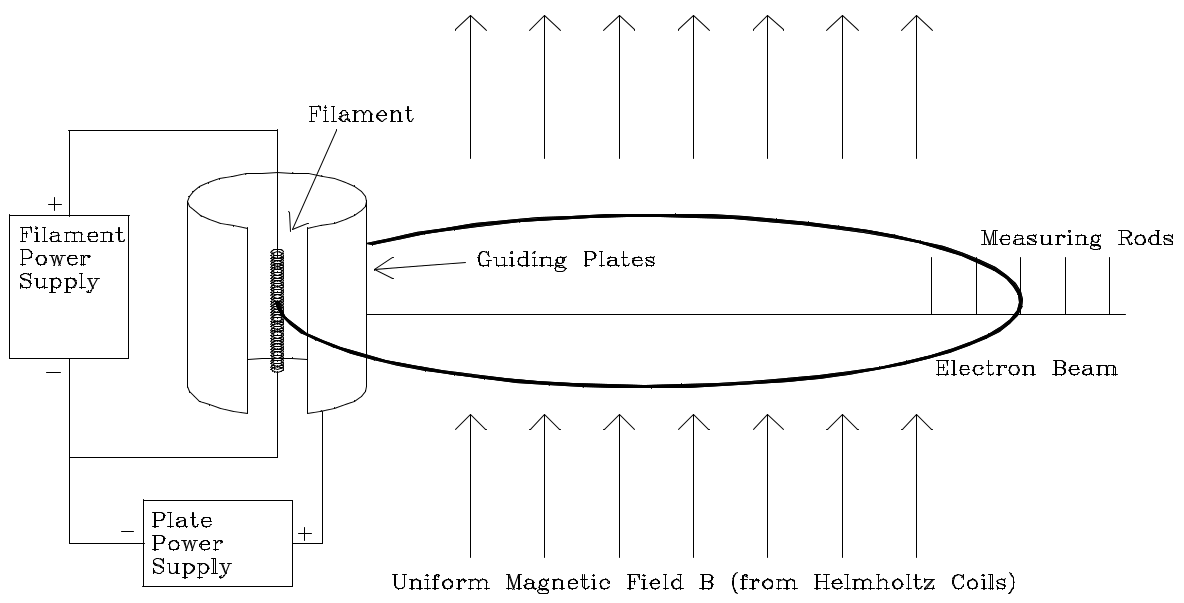
\includegraphics[width=0.8\textwidth]{./Exp6/pic/image1.png}
\caption{Converging Lens}
\end{figure}

\emph{Remark}: Sometimes lenses have a number printed on them which indicates the focal length, in millimeters. A positive number indicates a convex/converging lens while a negative number indicates a concave/diverging lens.\myskip

\emph{Remark for Experts}:  If a bundle of parallel rays falls on the lens but not along the axis of the lens, then the focal point will be shifted upward or downward along a line perpendicular to the axis (in the ``focal plane''). Note that the focal distance along the axis stays the same.
\begin{figure}[h]
\centering
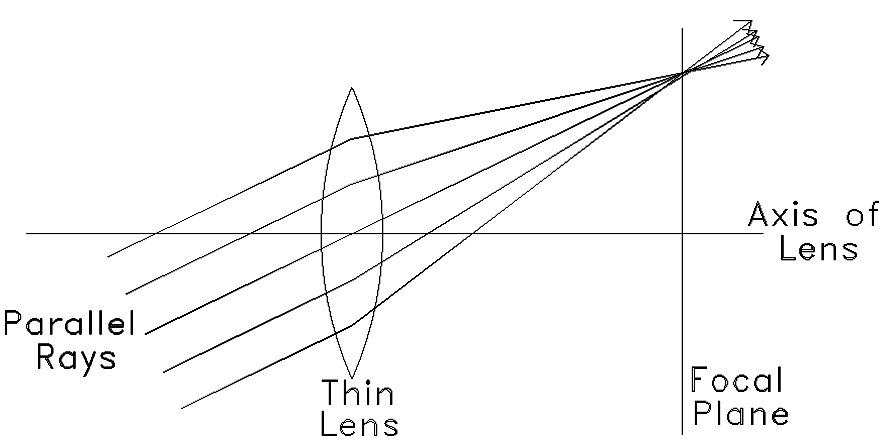
\includegraphics[width=0.6\textwidth]{./Exp6/pic/image2.png}
\caption{Focal Plane}
\end{figure}

\subsection{Ray Diagrams}
Ray diagrams allow us to trace the paths of rays. They make it easier to understand how images are formed and what lenses do. \myskip

To draw ray diagrams, follow a few simple rules illustrated in the figure below:
\begin{enumerate}
  \item Mark the focal points of the lens on each side of the lens.
  \item If two rays from a source point intersect at another point, then all rays from that source point will intersect at the second point.
  \item When drawing ray diagrams for convex lenses, it is most convenient to use three specific kinds of rays from the tip of the object ($P$) labeled $a$, $b$, and $c$ in the figure and described here:
  \begin{enumerate}
    \item Rays that enter the lens parallel to the axis pass through the focal point behind the lens.
    \item Rays that pass through the focal point in front of the lens leave the lens parallel to the axis of the lens.
    \item Rays going through the center of a lens will go through the lens in a straight line and do not bend. (These are the only rays that have no net refraction from the lens)
  \end{enumerate}
\end{enumerate}

\begin{figure}[h]
\centering
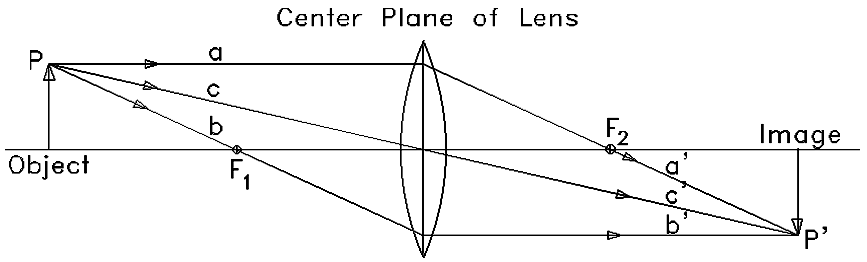
\includegraphics[width=0.8\textwidth]{./Exp6/pic/image3.png}
\caption{Ray Diagram}
\end{figure}

\subsection{Lens Equation}
\label{sec:lens}
The ray diagram described in the previous section provides a graphical method for locating images. Using the simple geometrical argument given here, with the notation indicated in Figure \ref{fig:lenseq}, we derive the lens equation. This equation relates the image distance $S'$, the object distance $S$, and the focal length $f$.
\begin{figure}[h]
\centering
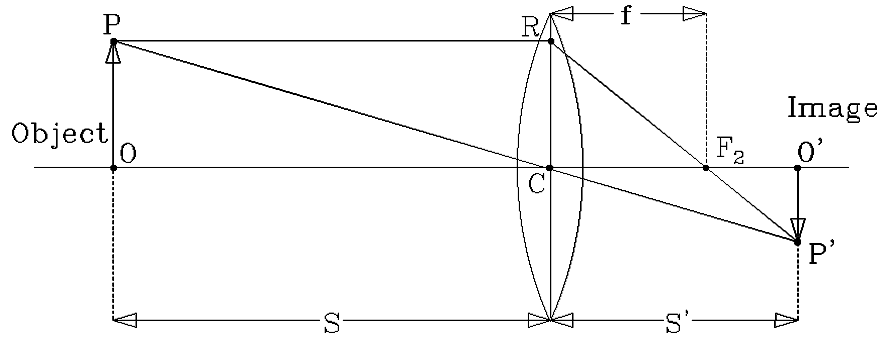
\includegraphics[width=0.8\textwidth]{./Exp6/pic/image4.png}
\caption{An image $P'$ of an object $P$ is formed by a lens}
\label{fig:lenseq}
\end{figure}

Since triangle $COP$ is similar to triangle $CO'P'$:
\begin{equation}
  \frac{S'}{S}=\frac{CO'}{CO}=\frac{O'P'}{OP}
  \label{eq:one}
\end{equation}

Since triangle $F_2O'P'$ is similar to triangle $F_2CR$:
\begin{equation}
  \label{eq:two}
  \frac{S'-f}{f}=\frac{O'F_{2}}{CF_{2}}=\frac{O'P'}{RC}=\frac{O'P'}{OP}
\end{equation}

Combining equations ({\ref{eq:one}}) and ({\ref{eq:two}}):
\begin{equation}
  \frac{S'}{S}=\frac{S'-f}{f}
\end{equation}
which reduces to:
\begin{equation}
  S'f=SS'-Sf
\end{equation}
and finally, dividing by $fSS'$ and rearranging, we obtain the thin lens equation:
\begin{equation}
  \frac{1}{f}=\frac{1}{S}+\frac{1}{S'}.
\end{equation}

The sign convention that we have used in deriving this equation, sets $f$ is positive for a converging lens, $S$ is positive on the side of the lens where the object is placed, and $S'$ is positive on the other side of the lens. Sign convention is \emph{incredibly important to understand for this experiment}. For $S>f$, $S'$ is also positive and a real image exists on the other side of the lens, as shown in the figure above. If the object were placed inside the focal length, i.e. if $S<f$, then the solution of the lens equation would give a negative value for $S'$ and the image would appear on the same side of the lens as the object.\myskip

The magnification of the image is the ratio of the image height to the object height. Eq. ({\ref{eq:one}}) shows that this magnification is numerically equal to $S'/S$, the ratio of image distance to object distance. The figure above also shows that the real image, formed when $S>f$, is inverted.

\section{Experiments}

\begin{figure}[h]
    \begin{center}
        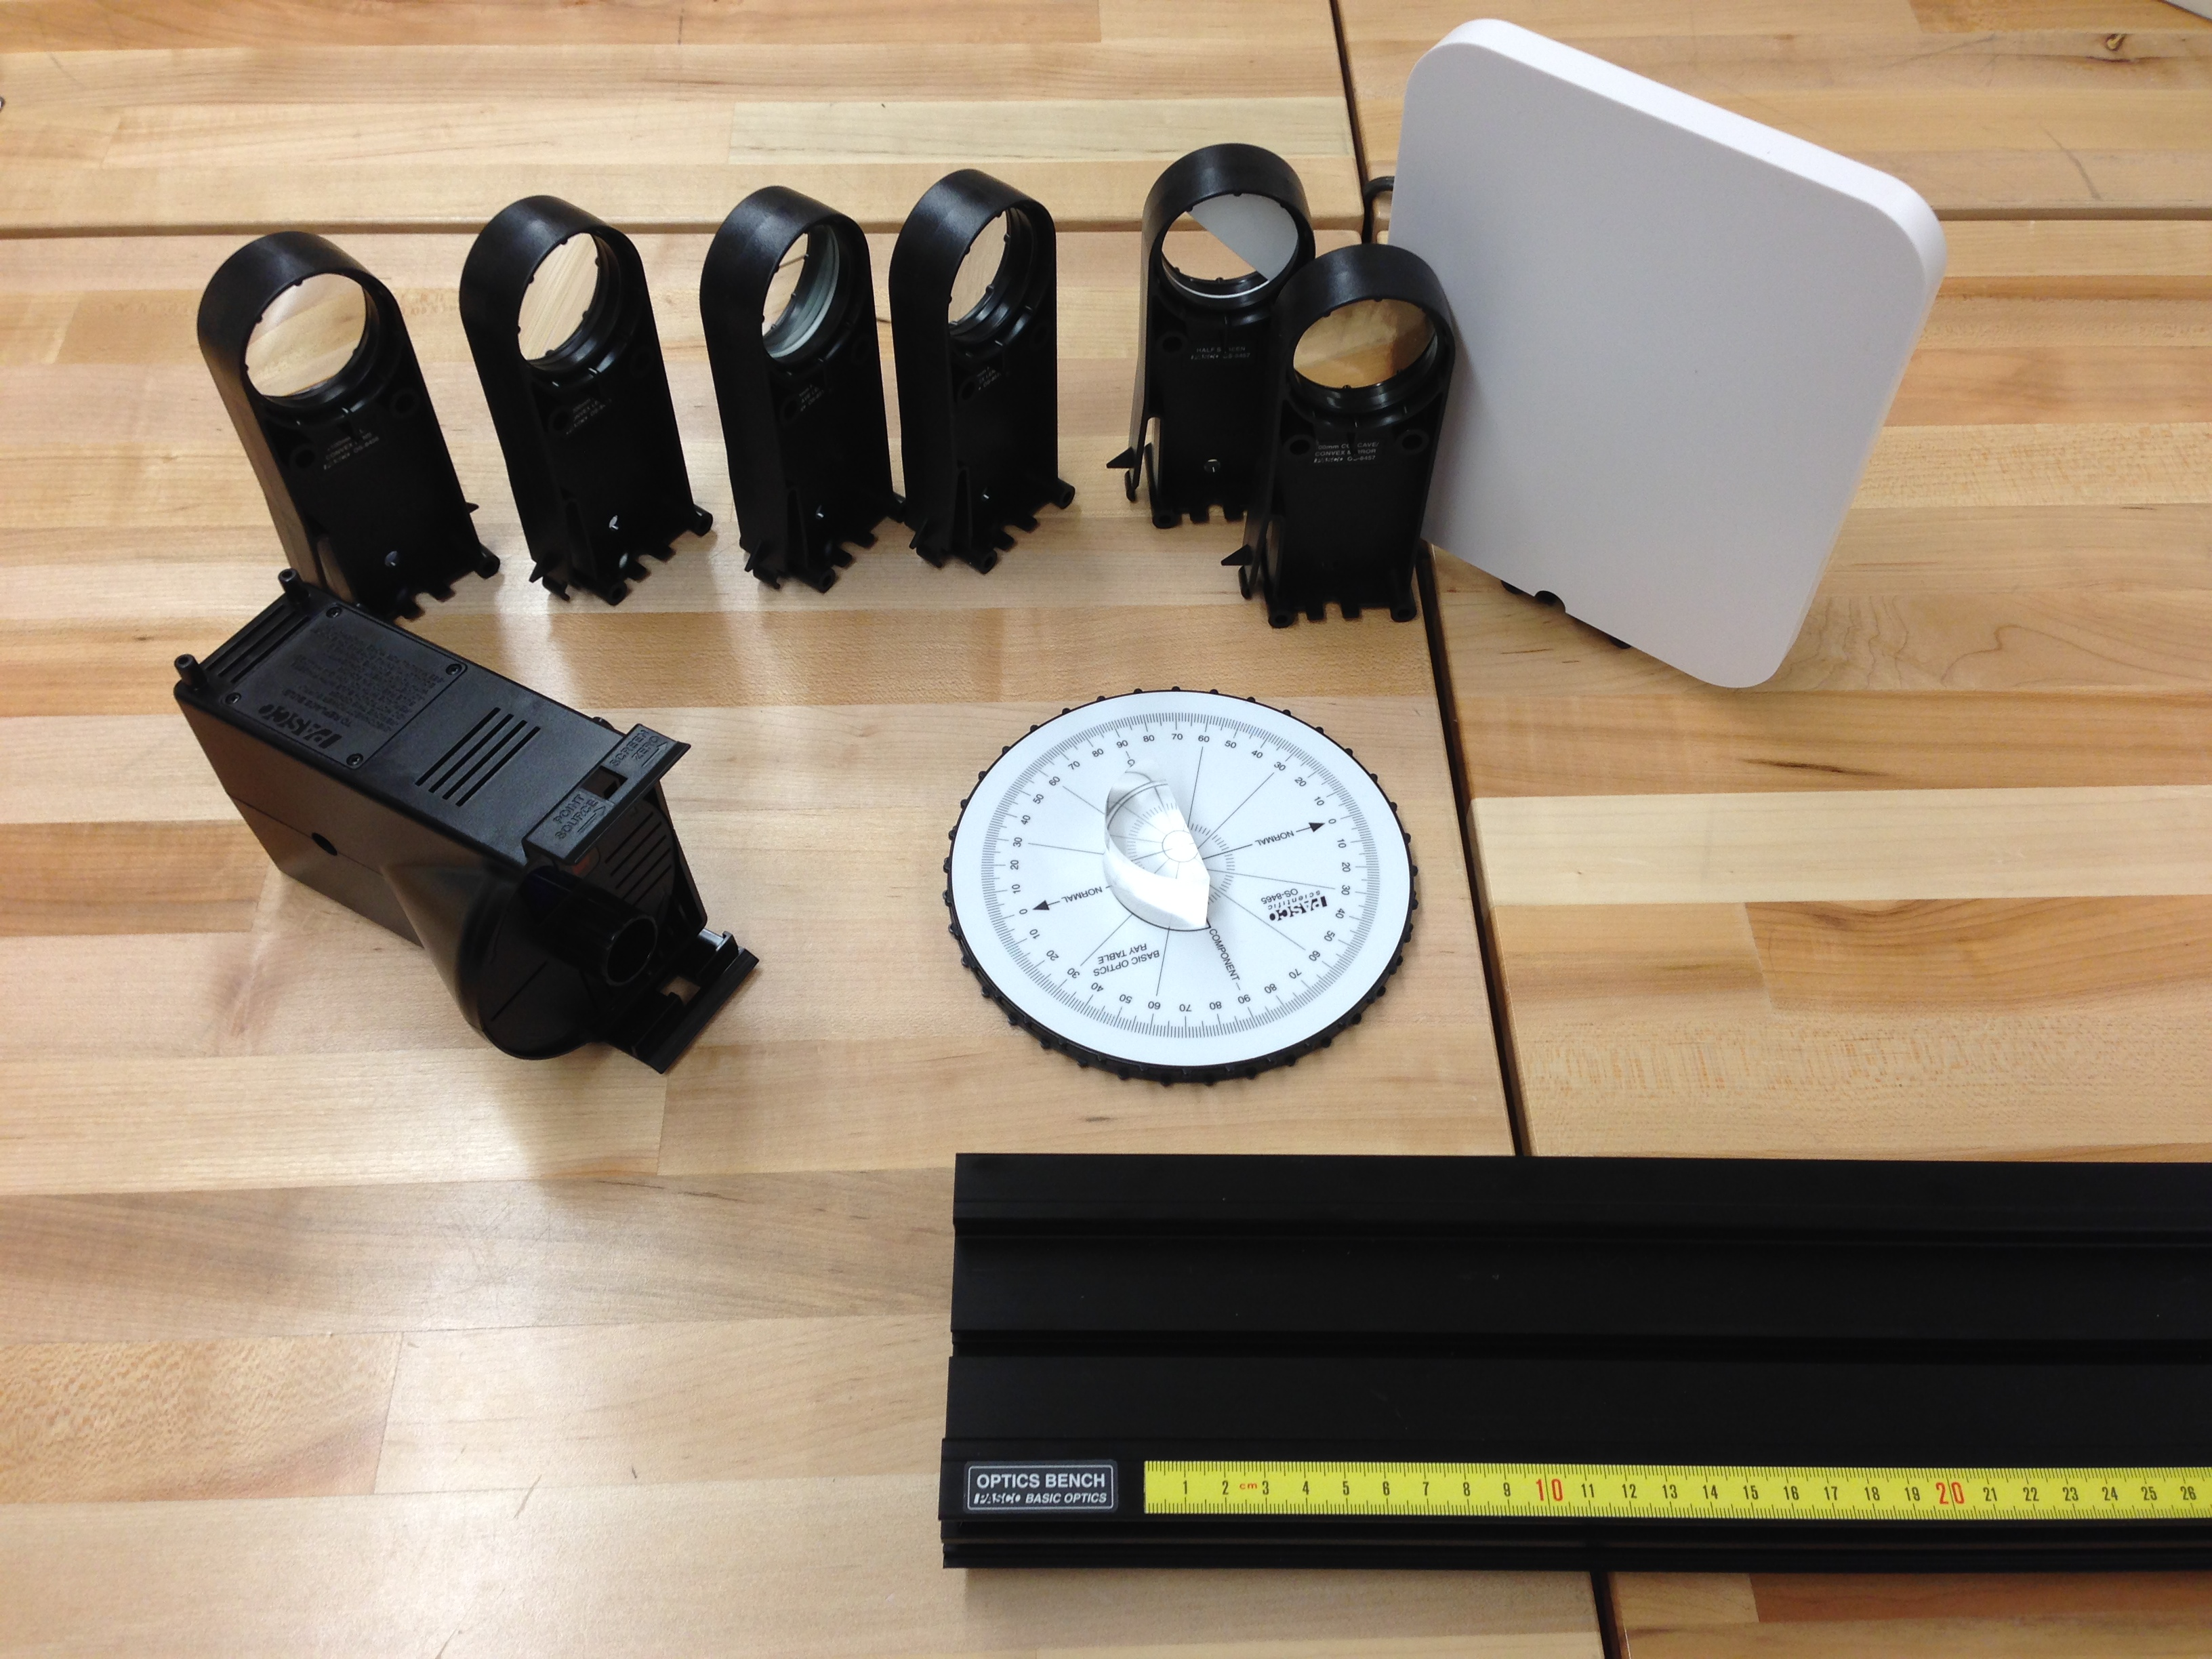
\includegraphics[width=0.8\textwidth]{./Exp6/pic/equipment.jpg}
    \end{center}
    \caption{Equipment for the Experiment}
    \label{fig:equip4}
\end{figure}

\subsection{Law of Reflection and Snell's Law}
\label{sec:refsnell}
In the first part of the lab we verify the Law of Reflection and Snell's Law with the materials seen in Figure ~\ref{fig:equip4}.  To begin, set the D-shaped acrylic lens in in the similarly-designed outline on the Ray Table.  Rotate the knob on the front of the Versatile Light Source until one light ray emerges, and arrange it so it perpendicularly crosses the flat side of the center of the acrylic lens (you can arrange it to align with the ``Normal" arrow on the Ray Table).  Now rotate the Ray Table such that the ray still crosses the center of the lens, but is no longer orthogonal, as in Figure \ref{fig:slaw}.  You should see transmitted and reflected rays.  Using the angle markings on the Ray Table, measure and record these angles along with that of the incident ray.  Repeat this process for two other incident angles.\myskip

\begin{figure}[h]
\centering
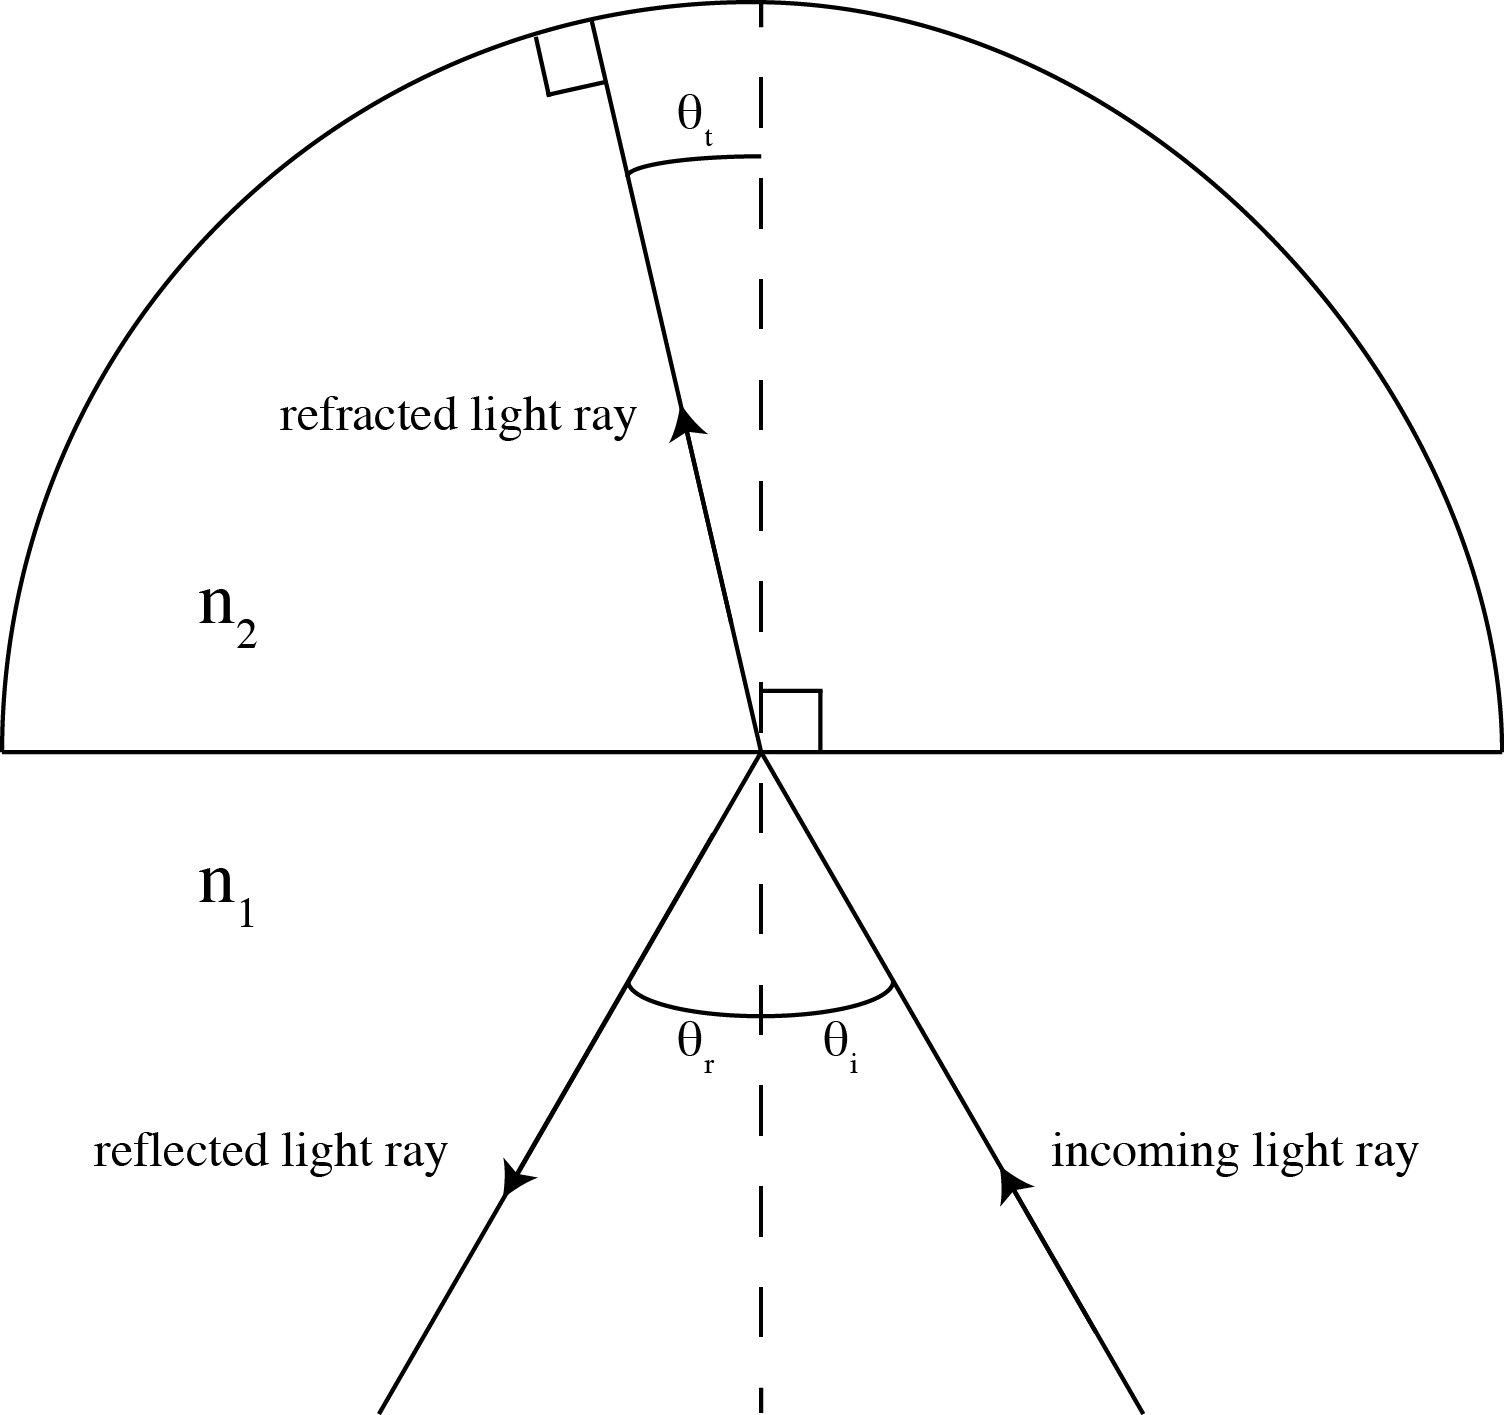
\includegraphics[width=0.8\textwidth]{./Exp6/pic/snelllawdiagram.png}
\caption{This diagram demonstrates what should happen as a bundle of light rays incident on the face of a D-shaped acrylic lens at angle $\theta_{i}$ are reflected and refracted at angles $\theta_{r}$ and $\theta_{t}$, respectively.}
\label{fig:slaw}
\end{figure}

Consider $\theta_{i}$ vs. $\theta_{r}$:
\begin{enumerate}
	\item Do the incident and reflected rays intersect at the reflecting edge of the acrylic?
	\item Estimate a reasonable uncertainty for these angles, considering the technique used to construct and measure them.
	\item Are the two angles equal within uncertainty?
	\item With Microsoft Excel, plot $\theta_{i}$ vs. $\theta_{r}$ with error bars and draw construct a best-fit line.
  \item Determine the slope and intercept of your best-fit line using the LINEST method. What would you expect for the values of the slope and intercept? Why?
  \item What were the main errors in performing this experiment?
\end{enumerate}
\myskip

\noindent{Consider $\sin \theta_{i}$ vs. $\sin \theta_{t}$:}
\begin{enumerate}
    \item Calculate the refractive index $n$ explicitly from each of the six pair of rays in your data. Calculate the mean and estimate the uncertainty of a single measurement using the 2/3 method.
    \item Does your measured index of refraction for acrylic agree with the accepted value of approximately 1.49 within error?
    \item Discuss the main sources of error in determining the index of refraction.
\end{enumerate}

\subsection{Total Internal Reflection and Critical Angle}

\begin{figure}[h]
\centering
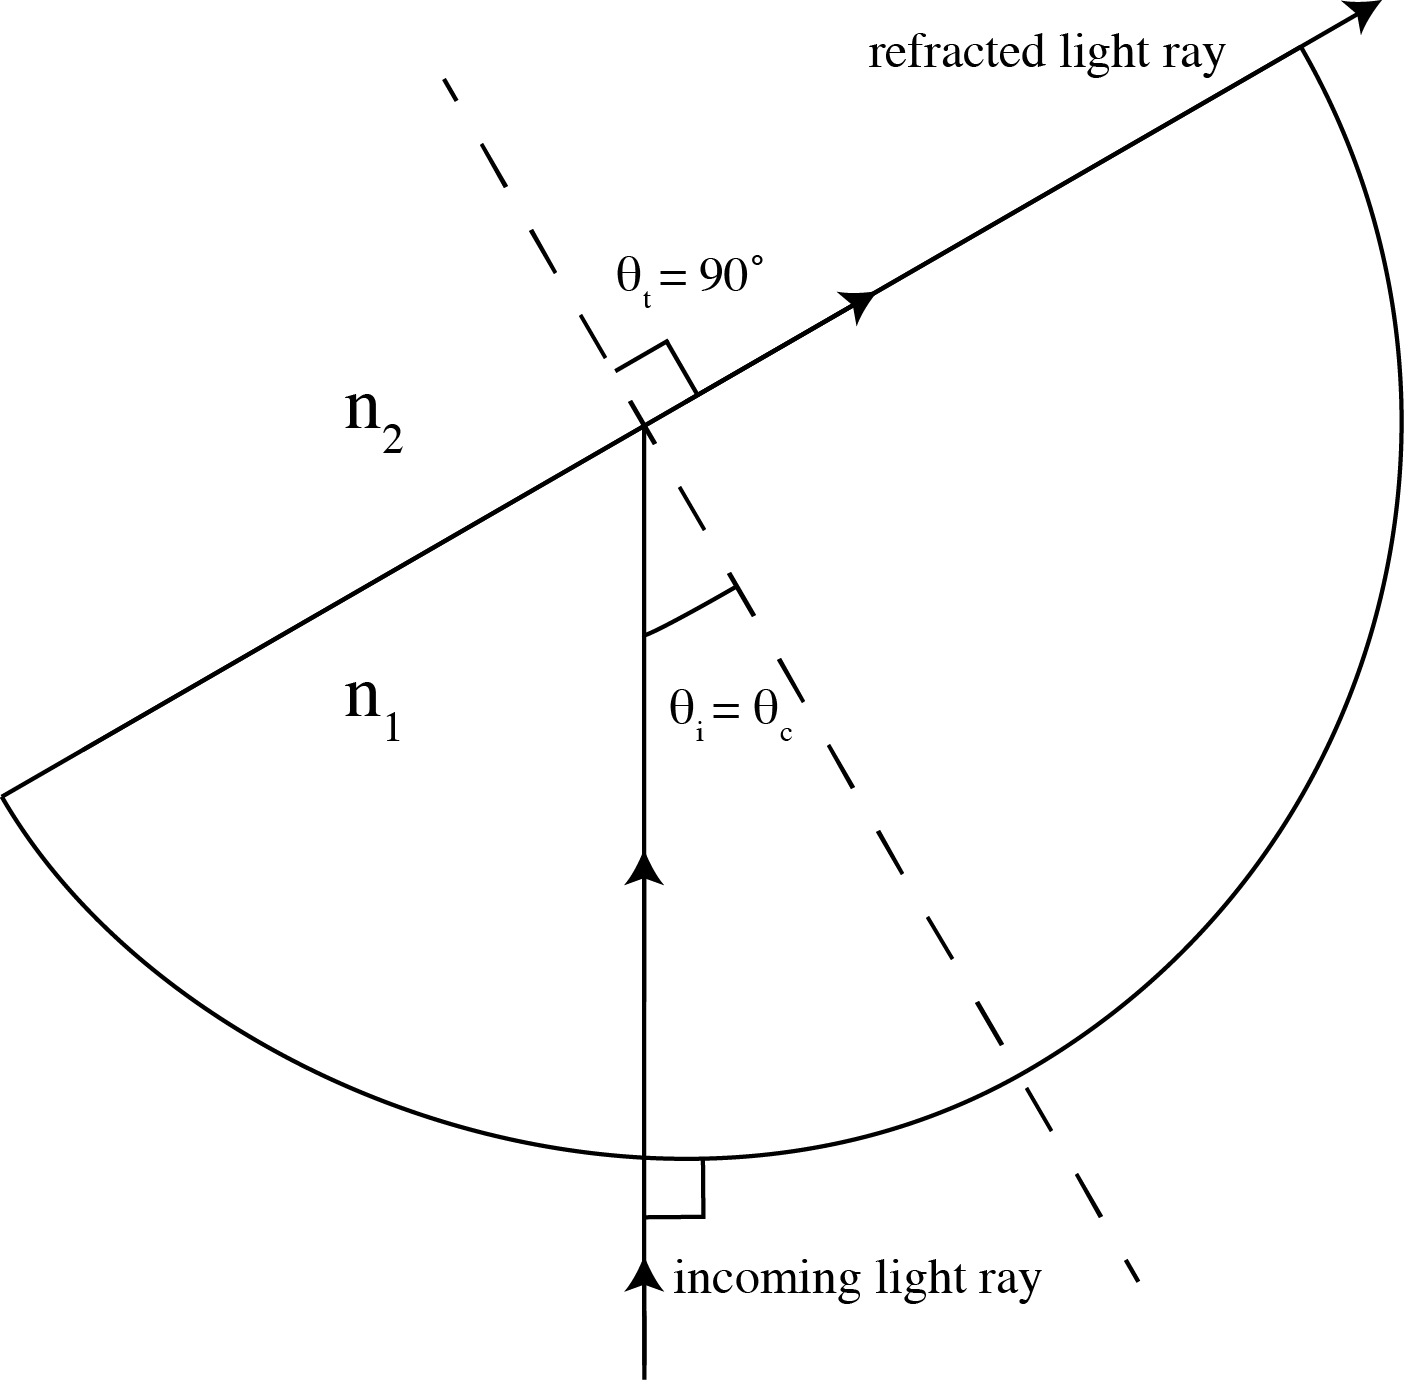
\includegraphics[width=0.8\textwidth]{./Exp6/pic/tirdiagram.png}
\caption{This demonstrates how one achieves total internal reflection in the case where $n_{1}>n_{2}$ and thus $\theta_{i}<\theta_{t}$.  Note because a line running from a circle's center to any point is necessarily orthogonal to the circumference, some simple geometry allows us to easily determine the $\theta_{i}$ that leads to the critical angle $\theta_{c}$.  It is recommended you study this figure until you are convinced of this.}
\label{fig:tirdiagram}
\end{figure}

In the previous section, we found $\theta_{i} > \theta_{t}$ as the light passed from air to acrylic (Snell's Law guaranteed this because $n_{\rm air} < n_{\rm acrylic}$).  Total internal reflection may only occur when light passes from a medium with a higher index of refraction to one with a lower ($n_{i} > n_{t}$).  For this portion of our experiment we want to setup a scenario in which light passes from acrylic to air.  Figure \ref{fig:tirdiagram} shows a schematic for how we can accomplish this.\myskip

Begin with the ray of light from the Versatile Light Source orthogonally penetrating the curved portion of the D-shaped acrylic lens along the "Normal" line that is transcribed on the Ray Table.  You should see the ray of light emerge perpendicularly to the flat surface of the acrylic along the opposite side's ``Normal" tracing.  Next begin rotating the Ray Table.  In doing so, you should notice the emerging ray of light from the acrylic's flat side begins to bend.  Though the effect is initially subtle, eventually you should reach an angle where the refracted light is now at $\theta_{t}=90^{\circ}$.  This incident angle has reached the critical angle $\theta_{c}$ - the point beyond which we have total internal reflection, and no refracted light escapes from the acrylic.

Measure the angle $\theta_{c}$ at which total internal reflection occurs.
\begin{enumerate}
    \item   From $\theta_{c}$ determine the index of refraction for the acrylic lens with error.  Error can be found by propagating uncertainty in $\theta$ using
    \begin{equation}
      \sigma_{\sin(\theta)} = \cos(\theta) \sigma_\theta
    \end{equation}
    \item	Does this value for $n$ agree with your findings in Section \ref{sec:refsnell} and with the accepted value within error?
    \item Discuss the main sources of error in measuring the index of refraction in this section.
\end{enumerate}

\noindent{\emph{An alternate way to achieve total internal reflection}: Begin with the ray of light from the Versatile Light Source orthogonally aligned with the flat face of the D-shaped acrylic lens, as we did with Snell's Law.  This time instead of rotating the Ray Table, simply slide it sideways so that the light beam remains perpendicular to the flat face of the lens, but now crosses on either the left or right side of the center.  You should notice that the light ray remains perpendicular to the face once in the acrylic.  However, it will now hit the curved portion of the D-shaped lens at an angle less than $90^{\circ}$, and as a result is refracted out the back.  Eventually you will reach a distance where you notice the light is no longer refracted, but appears to bounce around the circular portion of the lens, due to recurring total internal reflections.}\myskip

\subsection{Measuring the Focal Length of a Lens}
\label{sec:lengthI}
\begin{figure}[h]
\centering
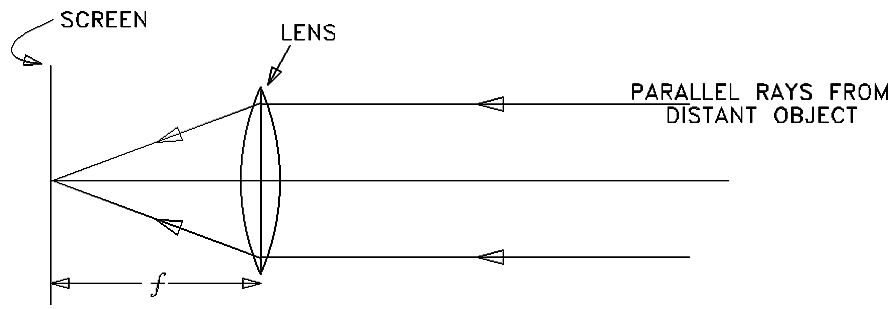
\includegraphics[width=0.7\textwidth]{./Exp6/pic/image8.png}
\caption{Measuring the Focal Length}
\label{fig:focusedray}
\end{figure}
Using a lens and a piece of paper, focus the image of an object outside the laboratory window (such as a tree or light outside the window) onto the paper, like illustrated in Figure \ref{fig:focusedray}.  If it is dark outside or the window blinds are closed, you can use a lightbulb in the room. Based on the fact that light from a distant source may be safely assumed to contain only parallel rays, the distance between the lens and the paper should be the focal length of the lens. You may already suspect that this method is not very precise and that you will get large uncertainties.

\begin{enumerate}
\item Measure this distance and estimate uncertainty for two lenses of your choosing.
\item Take note of the orientation of the image on your paper.
\item How could you improve this simple procedure?
\end{enumerate}

\subsection{Lens Equation}
\label{sec:lensequation}

Set up your optical bench in the following way: stand the Versatile Light Source upright on one end of the optical bench such that the crossed arrow target points down the bench. Place one convex lens on the bench a distance that is greater than its focal length $f$ from the Light Source.  Finally, place the Viewing Screen on the opposite side of the lens and move it forward and backward until the crossed arrow target comes into focus. By measuring $S$ and $S'$, you can verify the lens equation.
\begin{enumerate}
\item Repeat this measurement of $S$ and $S'$ for four more initial positions of the lens, each time readjusting the screen until the new arrow is clear. Be sure to include uncertainties.
\item With Microsoft Excel, plot $1/S'$ vs. $1/S$, with error bars. Draw a best-fit line and determine the slope and intercept with the LINEST method. You should be able to determine the focal length $f$ from the intercept!
\item Is your value of $f$ consistent with your value from the previous measurements? Is the value of the slope of the line what it is supposed to be?
\item Comment on how well the line fits your data points.
\item Which of the two methods used so far should give you the best estimate for $f$? Explain why.
\item Discuss the main sources of error in determining $f$. How would you improve this experiment?
\end{enumerate}

\section{Applications}

\emph{Swimming pool experience}:\vspace{0.6\baselineskip}

The next time you go swimming, do the following experiment (safely!):\myskip

From underwater, look at people or trees outside the water. You will see that you can see them when you view with your eyes at small angles relative to the \underline{normal} to the water surface. But as you look at larger angles, you find that the water surface suddenly appears weird, somewhat like liquid mercury. This occurs because the water surface reflects like a mirror so that you are not able to observe anything outside the pool. This is a consequence of total internal reflection. (If you will not be swimming for a while, you can also check this by looking at the water-air surface of a fish tank from below.)\vspace{0.6\baselineskip}

\noindent\emph{Medical diagnoses}:\vspace{0.6\baselineskip}

A standard method of medical imaging utilizes ultrasonic sound echocardiography: ultrasonic sound waves produce images of inner body organs (along with many other applications). A wave of ultrasonic sound sent into the body is refracted and reflected as it passes through parts of the body of different density. The wave reflected from a specific organ is observed by a detector and produces an image. The manner in which the ultrasonic sound waves get reflected and refracted is similar to the case for light that we have considered.\myskip

An important difference between light and sound waves is that sound waves propagate faster in water than in air. (With light, it is the other way around!)  This means that, for sound, water has a lower refractive index than air! Therefore, total internal reflection occurs going from air to water.  To enable the sound waves to get into the body requires having no air between the source and the body, usually accomplished by putting a layer of gel between the sound head and the body. This also means you cannot send ultrasonic sound through air-filled organs (like the lungs).

The picture below shows an echocardiogram of a human heart:
\begin{figure}[h]
    \begin{center}
        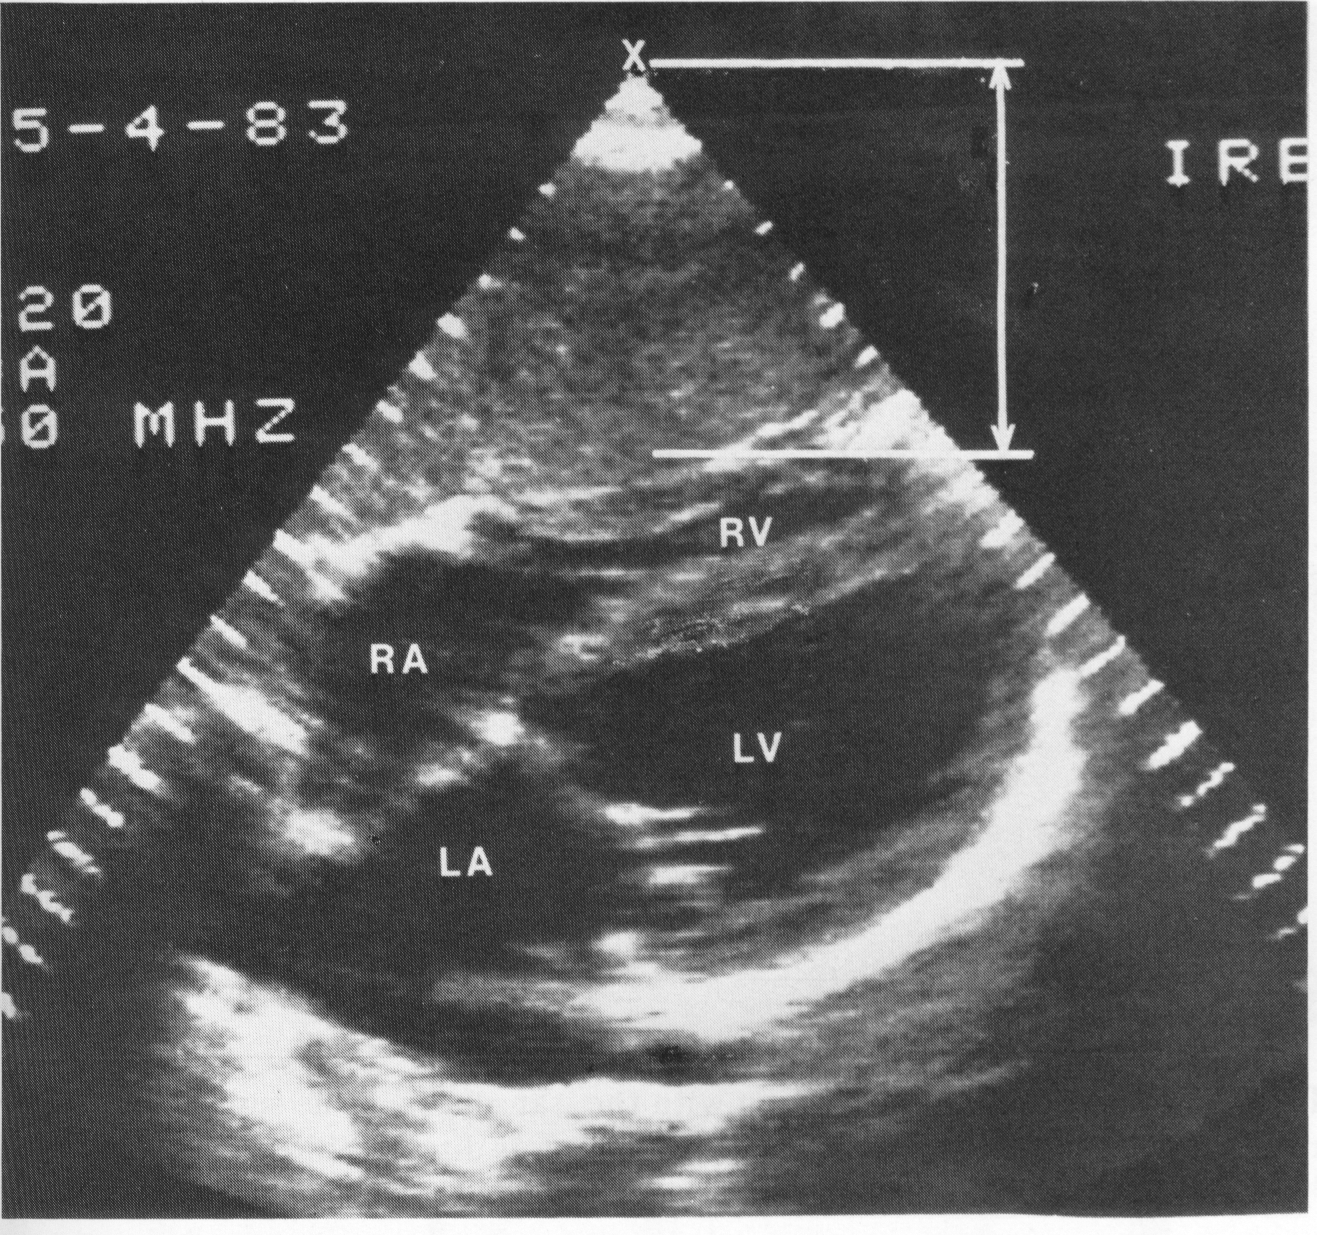
\includegraphics[width=0.5\textwidth]{./Exp6/pic/image021.png}
    \end{center}
    \caption{Echocardiogram of a Human Heart}
    \label{fig:heartgram}
\end{figure}

LA = left atrium, LV = left ventricle, RA = right atrium, RV = right ventricle.\myskip

(Picture from: Marvin Berger: Doppler Echocardiography in Heart Disease.)\myskip

\noindent\emph{The human eye}:\vspace{0.6\baselineskip}

The most important application of lenses (to us) is the human eye! The retina is located a fixed distance from the lens. We need the ability to focus objects located at different distances in front of the eye onto the retina. These specifications require us to have an adjustable lens (with variable focal length). Adjusting the focal length is accomplished by deformation of the lens through contraction of the ciliary muscles. If the eye views a distant object, the muscles are relaxed and the lens is rather flat, with a long focal length. If the eye must examine a nearby object, the muscles contract and the lens becomes rounder, with a shorter focal length. With advancing age, the lens loses its flexibility so that the eye loses much of its ability to adapt to objects at close distances. (A common misperception is that this can be compensated by ``eye exercises'', which would be the case if the problem were muscles. But the problem is not in lost vigor of the muscles, but in decreased flexibility of the lens!)\myskip

\begin{figure}[!h]
\centering
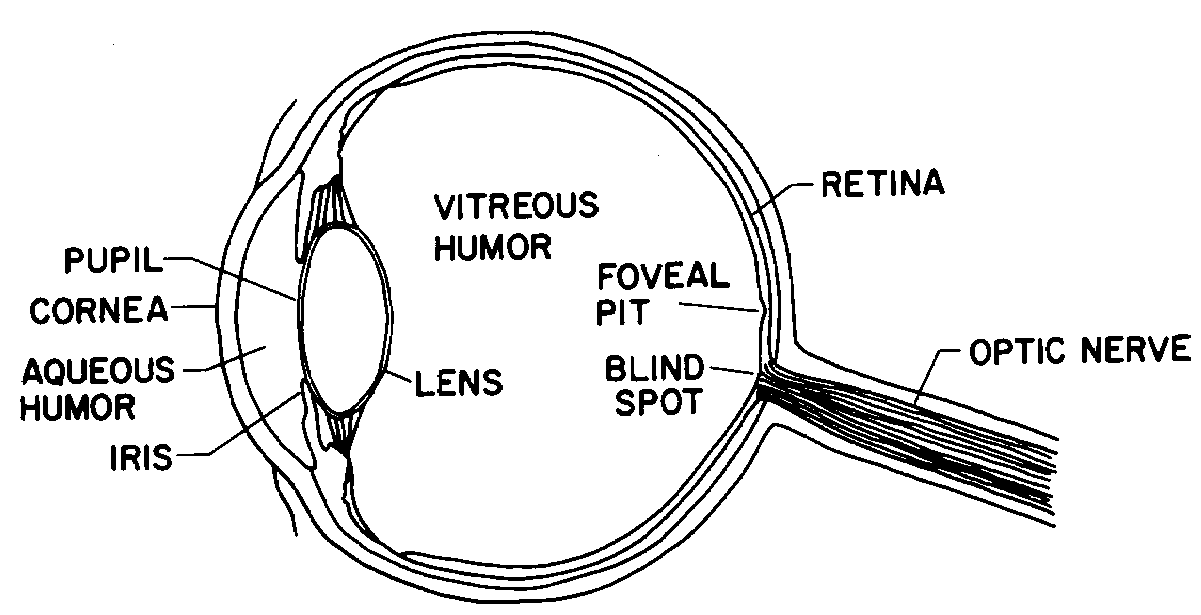
\includegraphics[width=0.7\textwidth]{./Exp6/pic/image11.png}
\caption{Human Eye}
\end{figure}

The two most common optical defects are nearsightedness and farsightedness. In a nearsighted (myopic) eye, the focal length is too short even when the ciliary muscles are completely relaxed. Thus, parallel rays from a distant object come to focus in front of the retina and fail to form a sharp image on the retina. Vision of distant objects is blurred. Eyeglasses with diverging lenses correct this condition. \myskip

In a farsighted (hyperopic) eye, the focal length is excessively long, even when the ciliary muscles are fully contracted. Hence, rays from a nearby object converge toward an image beyond the retina and fail to form a sharp image on the retina. Eyeglasses with converging lenses can correct this condition.\myskip

Reference: see Physics, by Ohanian, for further information.\myskip

Picture from: Daniel Malacara: Geometrical and Instrumental Optics.

\section{Lab Preparation Problems}

\noindent \underline{Absorption}:\myskip

1. How many times does a ray of light get reflected on a parallel pair of mirrors (which reflect $99\%$ of the incoming light) such that the total intensity is down to $50\%$? \myskip

\noindent \underline{Reflection}: \myskip

2. Explain in your own words the difference between specular and diffuse reflection using the following system and observations: \myskip

On a day with no wind, the surface of the sea can be very smooth and shiny. On the other hand, the tops of the waves appear white in a strong storm. \myskip

\noindent \underline{Refractive index and Snell's Law}:\myskip

3. What is the refractive index if a medium can slow down light to $v = 2/3\,\mathrm{c}$? \myskip

4. If you measure an incoming ray from the air to be at an angle of 15 degrees to the normal, what angle will it have in the medium with an refractive index of $n = 1.2$? \myskip

5. If you measure $\theta_{i} = 25$ degrees (air) and $\theta_{t} = 20$ degrees, what is the refractive index of the medium in which you measured $\theta_{t}$?\myskip

6. Given the following pairs of values for $\theta_{i}$ and $\theta_{t}$, draw a graph of $\sin \theta_{t}$ vs. $\sin \theta_{i}$. Determine the value of n using only the slope of the graph and not the individual values from the table.
\begin{table}[h]
    \centering
    \begin{tabular}{|l|l|l|l|l|l|}
        \hline
        $i$ in degrees & 0 & 15 & 30 & 45 & 60 \\ \hline
        $r'$ in degrees & 0 & 11.5 & 22.6 & 33.0 & 41.8 \\ \hline
    \end{tabular}
\end{table}

7. Given the following measured values for the refractive index, what is the mean and uncertainty (using the 2/3 rule)?
\begin{table}[h]
    \centering
    \begin{tabular}{|l|l|l|l|l|l|l|}
        \hline
        $n=$ & 1.24 & 1.21 & 1.29 & 1.23 & 1.27 & 1.26 \\ \hline
    \end{tabular}
\end{table}

\noindent \underline{Total Internal Reflection and Critical Angle}: \myskip

8. Given an refractive index of diamond $n = 2.42$, what is its critical angle? \myskip

9. You want to measure the refractive index of water. For that you take a glass of water or go to your fish tank and look upwards at the air-water boundary through the side of your glass. When look at the boundary with a small enough angle, the surface will be (almost) $100\%$ reflective and you cannot see out through the boundary. With this setup, you measure the critical angle to be 60 degrees. What does this data give for the refractive index of water? Is it the same as the value you find in books?
